\section{Error Analysis and Model Insights}
\label{sec:error_analysis_and_model_insights}

\paragraph{Error Analysis}
We randomly sample 97 erroneous records and conduct a error analysis of the best-performing model, GPT-4o. We classify the errors into 7 types (See \Cref{xsec:error_analysis} for detailed descriptions and qualitative examples) and show their distribution in \Cref{fig:error_distribution}.

\begin{figure}[t]
    \centering
    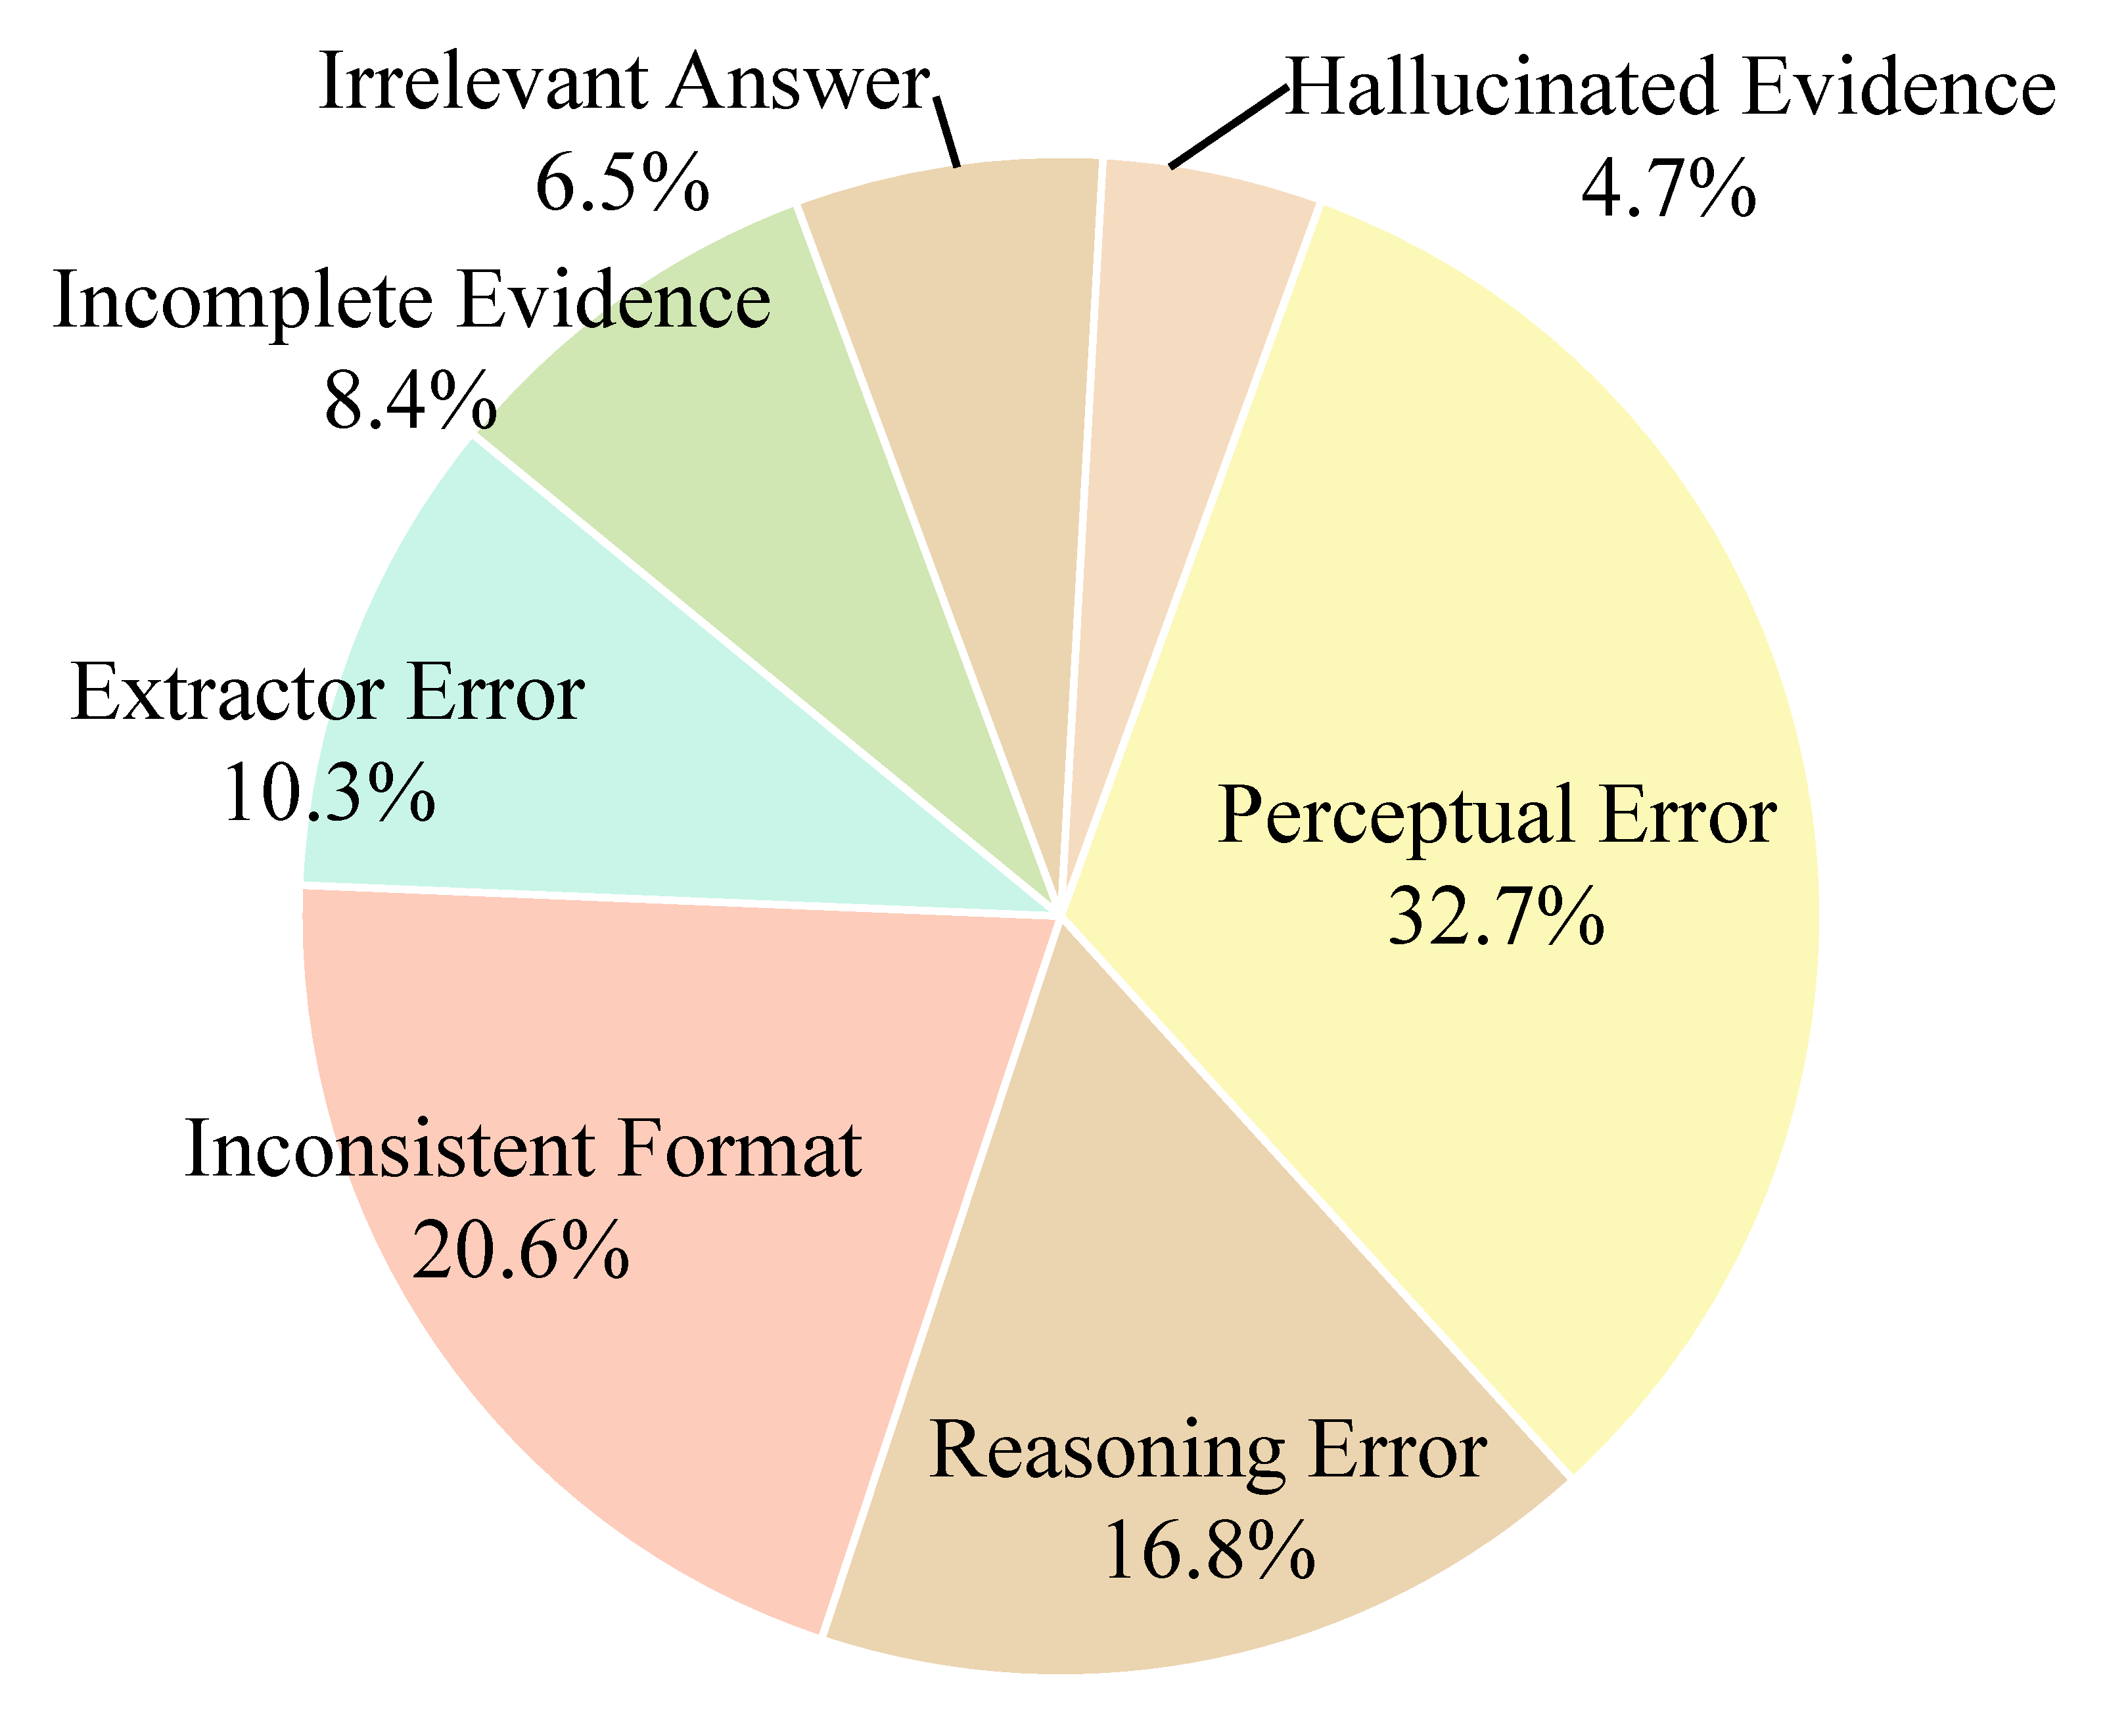
\includegraphics[width=0.42\textwidth]{img/error_distribution.pdf}
    \vspace{-0.1cm}
    \caption{Error distribution over 97 annotated GPT-4o errors.}
    \label{fig:error_distribution}
    \vspace{-0.5cm}
\end{figure}

\emph{Perceptual errors} constitute the most prevalent category (32.7\%), arising from inaccuracies in recognizing, parsing, or counting document elements such as tables, figures, and formulas. Typical manifestations include incorrect heading hierarchies and mismatched figure-text correspondences, indicating that complex document structures and OCR performance remain primary bottlenecks for LVLMs. An example of perceptual errors in LongDocURL is shown in \Cref{fig:perception_error_example_before_appendix}. \emph{Reasoning errors} represent the third-largest category (16.8\%), occurring during calculation, comparison, or summarization even when relevant evidence is correctly identified. A significant proportion of errors (20.6\%) involves \emph{inconsistent formats}, highlighting the inflexibility of rule-based evaluation. For instance, a response of "50212000" for "\$50.2 million" was incorrectly scored as entirely wrong. The remaining error categories (\emph{Hallucinated Evidence}, \emph{Irrelevant Answer}, \emph{Incomplete Evidence}, and \emph{Extractor Error}) collectively accounted for 29.9\% of cases.


\paragraph{Model Insights}
We analyze open-source models from two key aspects: \emph{dataset adaptation} and \emph{training strategy}. First, Qwen2-VL (LVLM) demonstrates superior performance over its LLM variant in \Cref{tab:main_results_1}, attributable to its extensive multimodal training that strengthens both comprehension and generation capabilities across modalities. Second, LLaVA-OneVision-Chat outperforms its base model (LLaVA-OneVision), as it employ Direct Preference Optimization (DPO) and human feedback to boost generalization and reasoning in long-document tasks. Additionally, we observe frequent failures caused by poor layout analysis and table/chart parsing. Incorporating layout parsing into continual pretraining or fine-tuning could mitigate these errors. Alternatively, a multi-stage response framework---where models first parse document structure before reasoning---may improve performance.

\begin{figure}[t]
    \vspace{0.3cm}
    \centering
    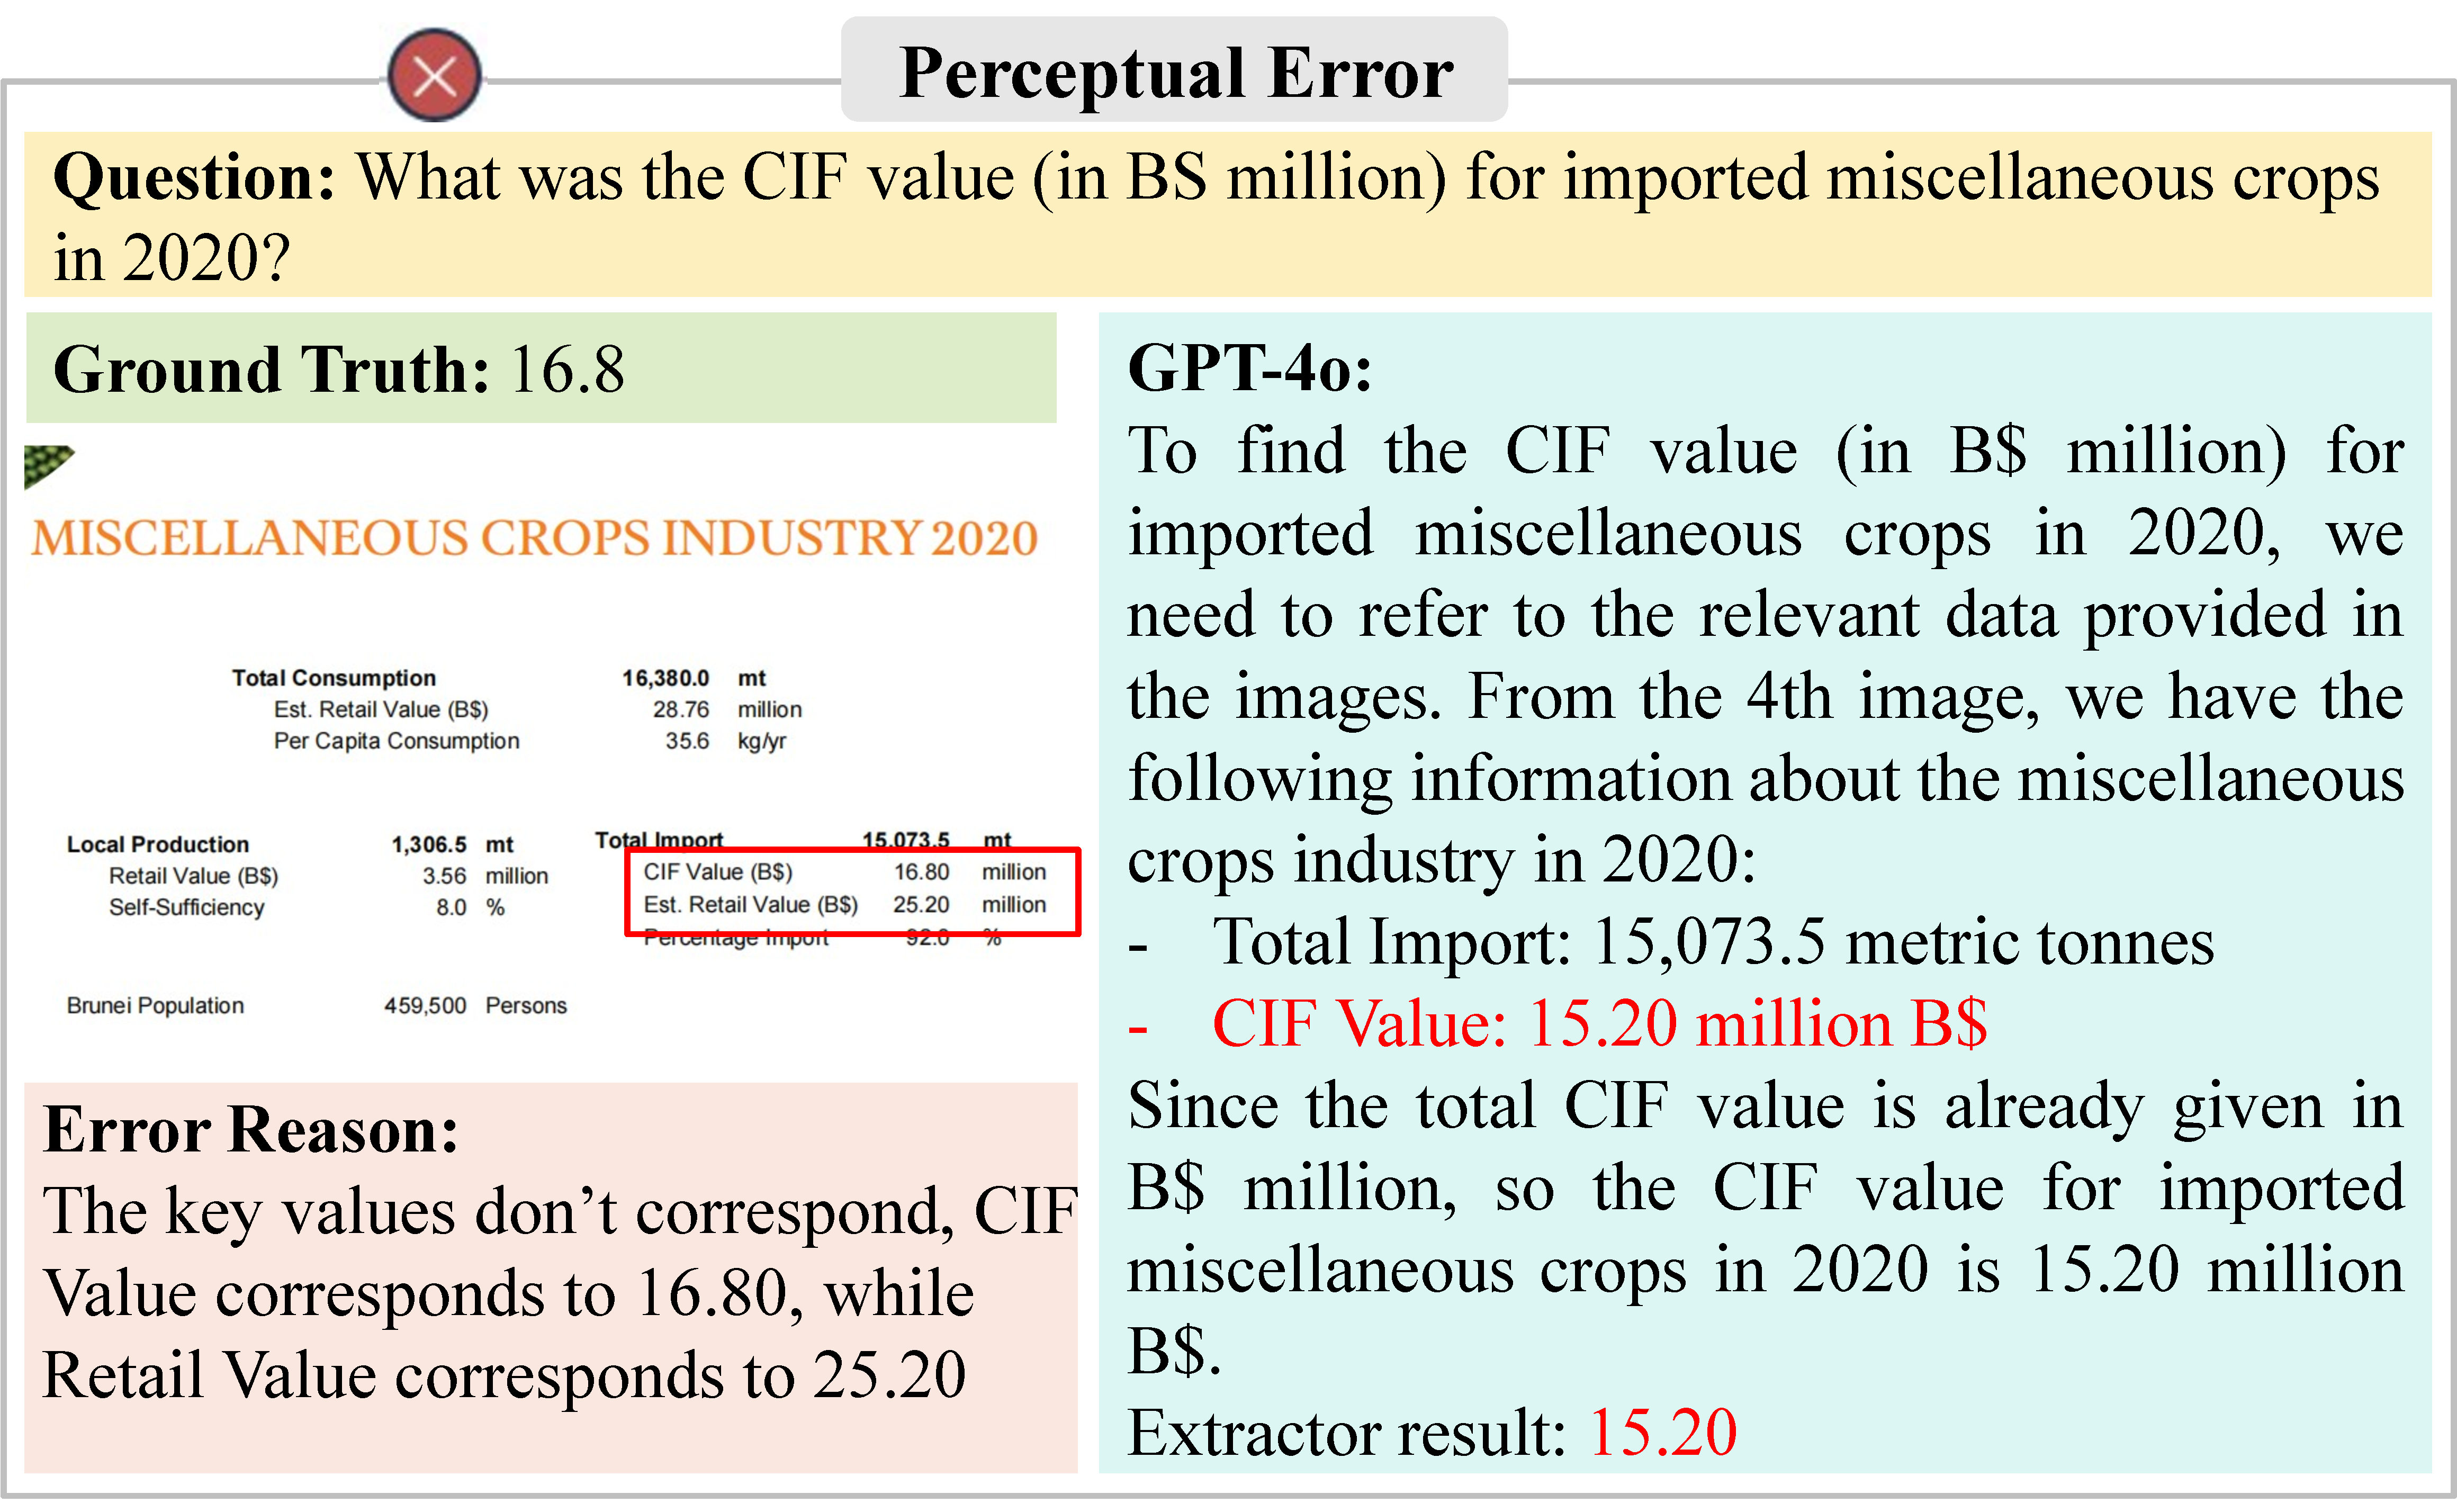
\includegraphics[width=0.50\textwidth]{img/perception_error_example_v2.pdf}
    \caption{A basic perception error, with the error highlighted in red.}
    \label{fig:perception_error_example_before_appendix}
    \vspace{-0.4cm}
\end{figure}